% Introduction
This section described the technologies used to query, cache, and process data in this project. Query engine refers mainly to Apache Spark and DuckDB, but also the other technologies presented in this chapter operate at the same abstraction level while having different functions.

\subsection{Apache Spark}

Apache Spark (from now on simply Spark) is an open-source distributed computing framework designed to handle large-scale data-intensive applications~\cite{zahariaApacheSparkUnified2016}. Spark builds from the roots of MapReduce and its variants. MapReduce is a distributed programming model first designed by Google that enables the management of large datasets~\cite{dean2004mapreduce}. The paradigm was later implemented as an open-source project by Yahoo! engineers under the name of Hadoop MapReduce~\cite{borthakurHadoopDistributedFile2005}. Spark improved this approach by making use of \glspl{RDD}~\cite{Zaharia:EECS-2011-82}. \glspl{RDD} are a distributed memory abstraction that enables a lazy in-memory computation that is tracked through the use of lineage graphs, ultimately increasing fault tolerance~\cite{Zaharia:EECS-2011-82}. The difference between Hadoop MapReduce and Spark is represented in Figure~\ref{fig:MapReducevsSpark}.

\begin{figure}[!ht]
  \begin{center}
    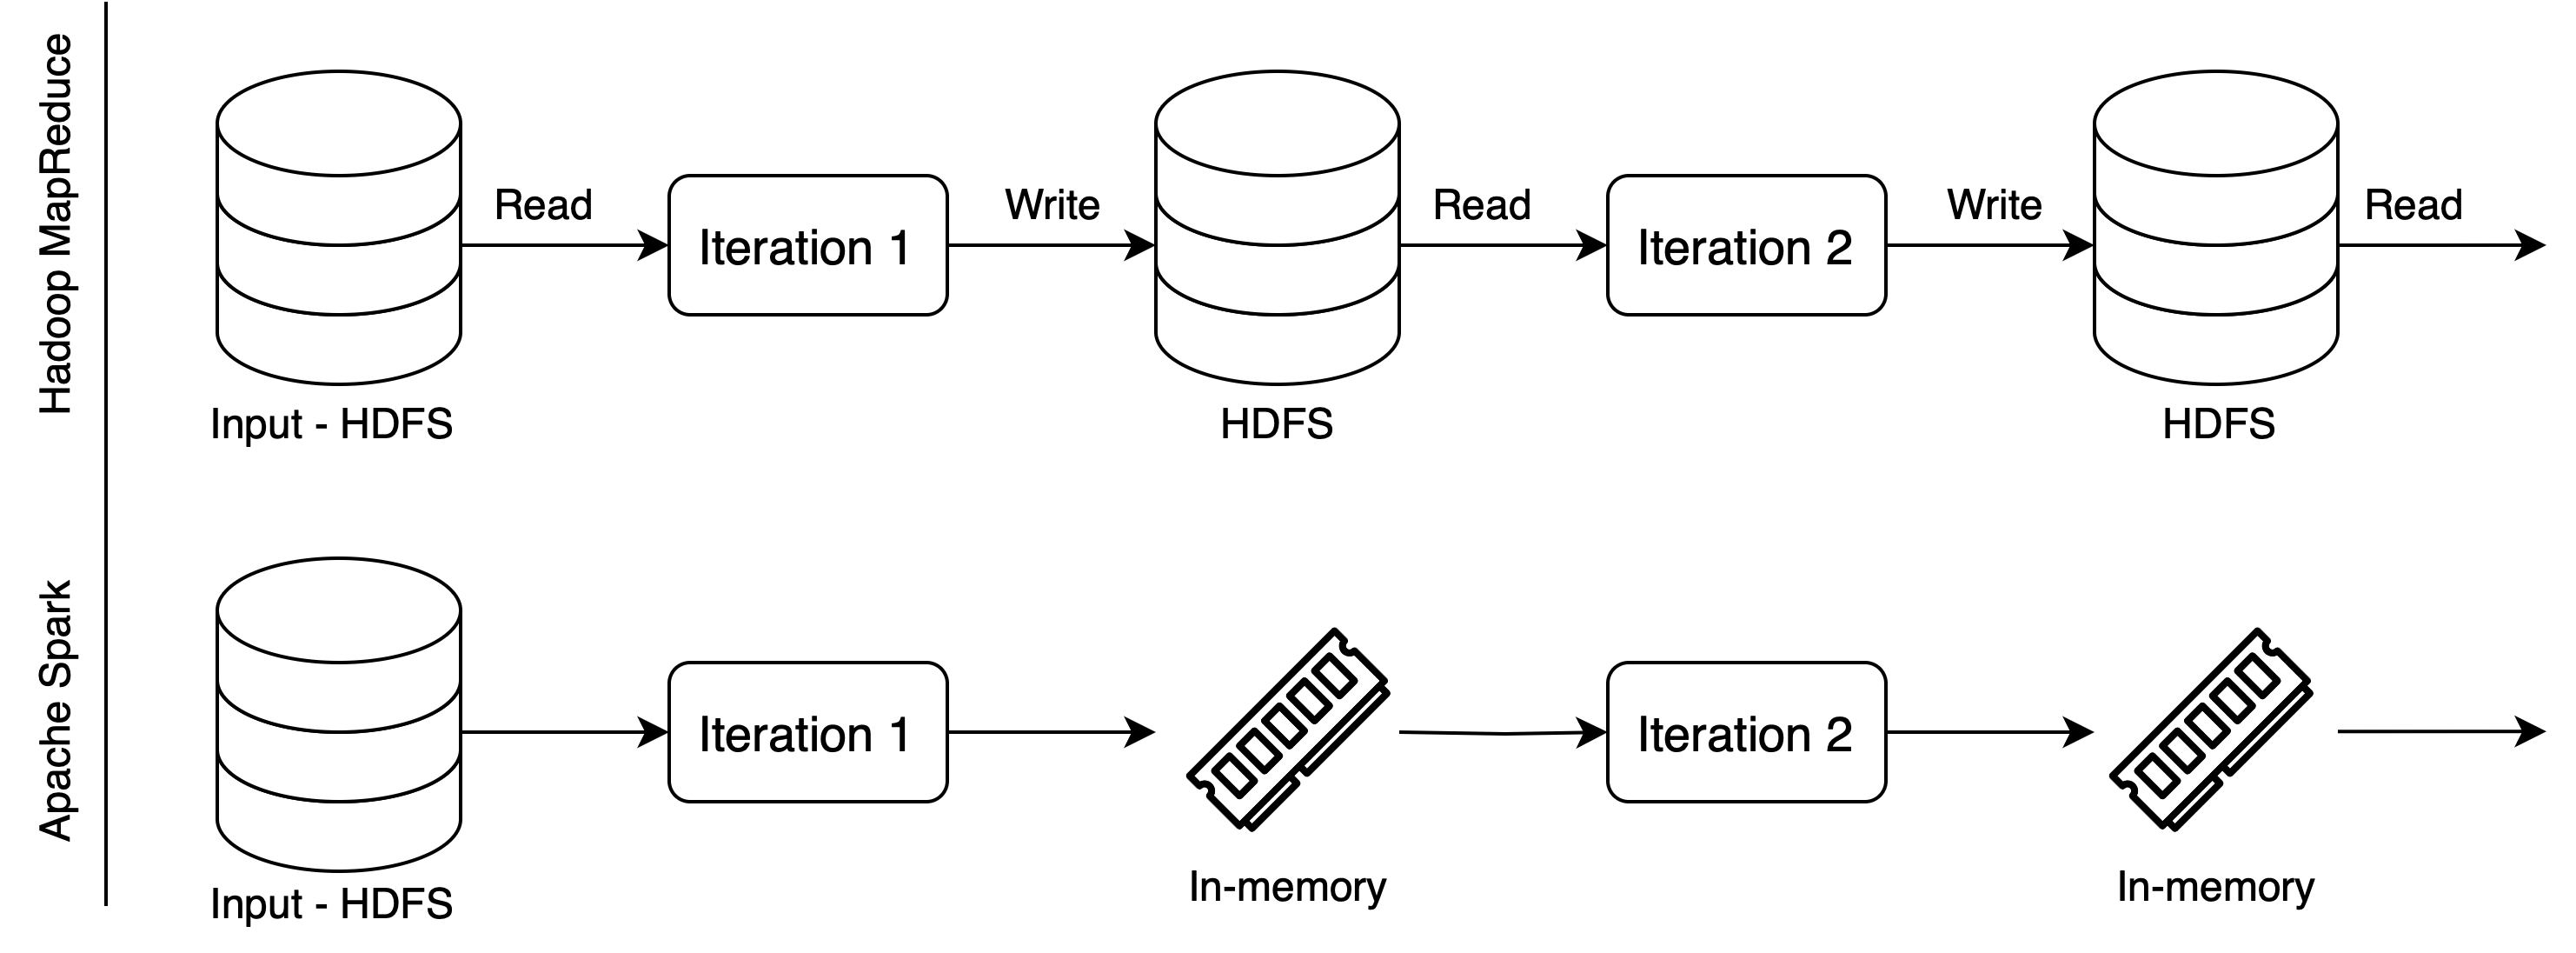
\includegraphics[width=\textwidth]{figures/2-background/Spark_MapReduce.png}
  \end{center}
  \caption{Hadoop MapReduce and Apache Spark execution differences}
  \label{fig:MapReducevsSpark}
\end{figure}

\subsection{Apache Kafka}

Apache Kafka (from now on, Kafka) is an open-source distributed data streaming platform designed for high-throughput, and scalable data processing~\cite{krepsKafkaDistributedMessaging2011}. Kafka is most typically used for real-time streaming applications thanks to low latency. 

\begin{figure}[!ht]
    \begin{center}
      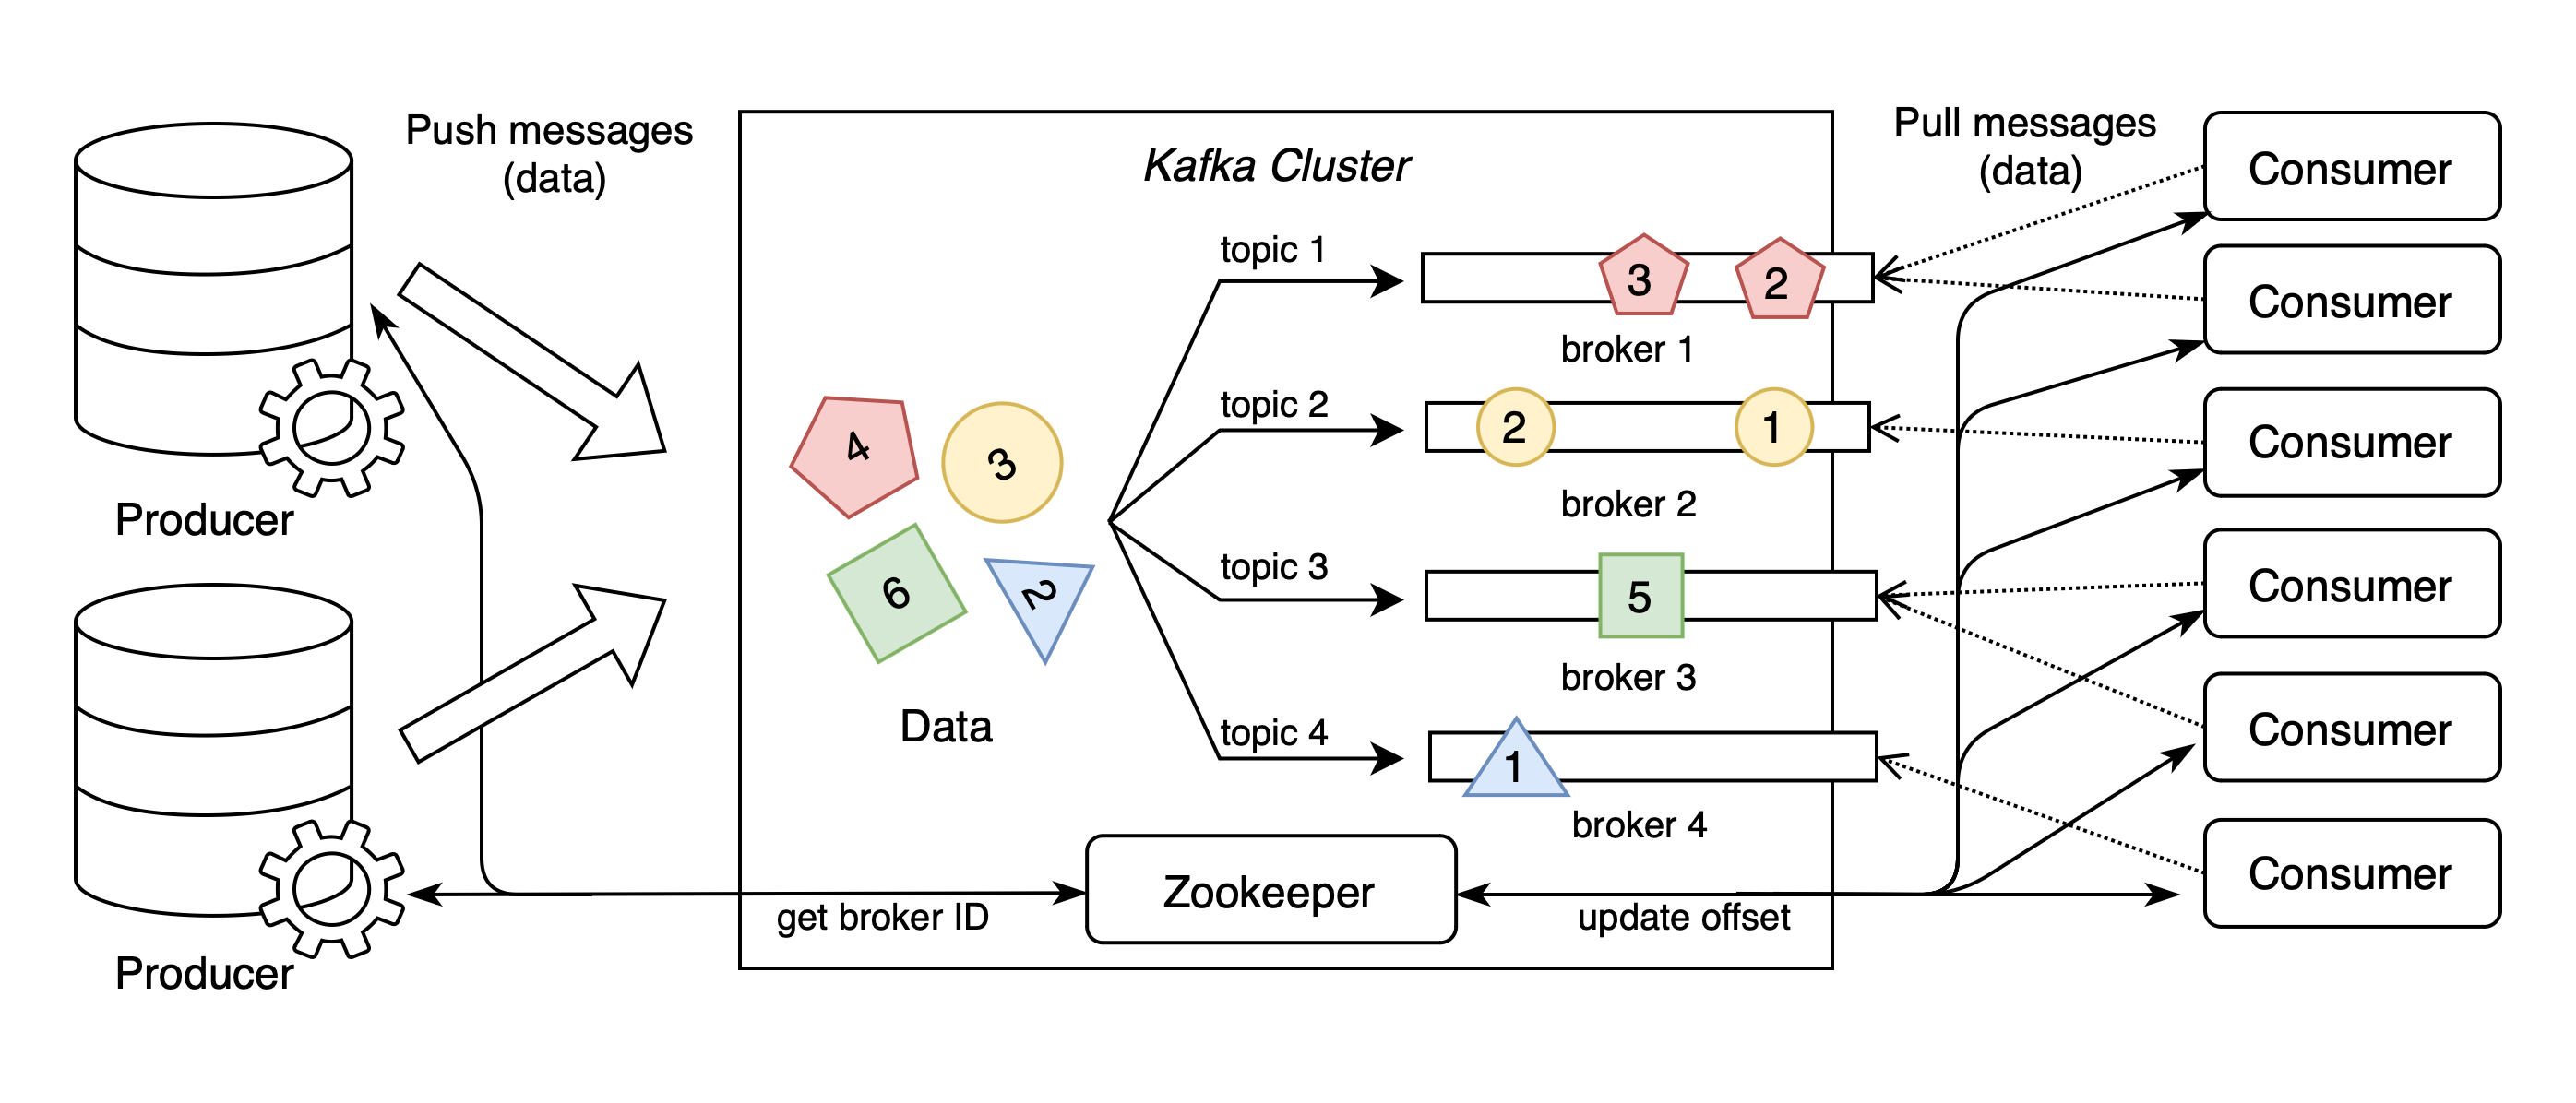
\includegraphics[width=\textwidth]{figures/2-background/kafka.png}
    \end{center}
    \caption{Kafka cluster}
    \label{fig:kafka}
\end{figure}

Figure \ref{fig:kafka} shows the components and messages exchanged in a Kafka cluster. The key components of Kafka are:
\begin{enumerate}
    \item \textbf{Producer}: an application that produces and labels data with specific topics (shapes in the figure).
    \item \textbf{Zookeeper}: responsible for keeping track of brokers and the topic's current offset.
    \item \textbf{Broker}: a computational node (or server) that handles data on a specific topic. It is responsible for receiving messages from producers. Once messages are received the broker forwards them on request by the consumers. This enables the asynchronous protocol.
    \item \textbf{Consumer}: an application that is interested in topic-specific data. To access data it is subscribed to a topic receiving new messages when published. To a topic, more consumers can be subscribed.
\end{enumerate}

The protocol allows applications acting as producers and consumers to avoid having a synchronous protocol. This enables producer's high throughput since they can send messages without waiting for consumers to process them. This also allows consumers to be flexible on workload size.

Given its distributed nature, Kafka allows several producers, consumers, and brokers to exist at the same time. This enables the system to be tuned according to the needs of a specific application. 

\subsection{DuckDB}

DuckDB \cite{raasveldtDuckDBEmbeddableAnalytical2019} is an open-source, embedded, \gls{OLAP} \gls{DBMS}. DuckDB was designed to process small quantities of data (1 - 100 GBs) within the same process or application that runs it, instead of a different process/application. These features create an efficient \gls{OLAP} database that can be used for data analysis, and data processing on a small scale, without the complexity of a more complex \gls{DBMS}, e.g. Teradata \cite{shahImproveYourOLAP}. 

The light structure that characterizes DuckDB is what enables this system to be extremely responsive with low latency. The limitations of the system regard data size, as DuckDB makes use of in-memory processing, it is not able to handle big workloads (1TB or more), which require multiple disk loads.

\subsection{Arrow Flight}

Arrow Flight is a high-performance framework for data transferring over a network, most typically Arrow tables \cite{wesmIntroducingApacheArrow2019}. This protocol enables the transfer of large quantities of data stored in a format, e.g. Arrow tables, without having to serialize or deserialize it for transfer. This speeds up the data transfer by a large margin making Arrow Flight extremely efficient. Arrow Flight is designed to be cross-platform, having support for multiple programming languages (C++, Python, Java). The protocol also supports parallelism, speeding up transfers by using multiple nodes on parallel systems. Arrow Flight protocol is built on top of gRPC, enabling standardization and an easier development of connectors. 